% Options for packages loaded elsewhere
\PassOptionsToPackage{unicode}{hyperref}
\PassOptionsToPackage{hyphens}{url}
%
\documentclass[
]{article}
\usepackage{amsmath,amssymb}
\usepackage{iftex}
\ifPDFTeX
  \usepackage[T1]{fontenc}
  \usepackage[utf8]{inputenc}
  \usepackage{textcomp} % provide euro and other symbols
\else % if luatex or xetex
  \usepackage{unicode-math} % this also loads fontspec
  \defaultfontfeatures{Scale=MatchLowercase}
  \defaultfontfeatures[\rmfamily]{Ligatures=TeX,Scale=1}
\fi
\usepackage{lmodern}
\ifPDFTeX\else
  % xetex/luatex font selection
\fi
% Use upquote if available, for straight quotes in verbatim environments
\IfFileExists{upquote.sty}{\usepackage{upquote}}{}
\IfFileExists{microtype.sty}{% use microtype if available
  \usepackage[]{microtype}
  \UseMicrotypeSet[protrusion]{basicmath} % disable protrusion for tt fonts
}{}
\makeatletter
\@ifundefined{KOMAClassName}{% if non-KOMA class
  \IfFileExists{parskip.sty}{%
    \usepackage{parskip}
  }{% else
    \setlength{\parindent}{0pt}
    \setlength{\parskip}{6pt plus 2pt minus 1pt}}
}{% if KOMA class
  \KOMAoptions{parskip=half}}
\makeatother
\usepackage{xcolor}
\usepackage[margin=1in]{geometry}
\usepackage{color}
\usepackage{fancyvrb}
\newcommand{\VerbBar}{|}
\newcommand{\VERB}{\Verb[commandchars=\\\{\}]}
\DefineVerbatimEnvironment{Highlighting}{Verbatim}{commandchars=\\\{\}}
% Add ',fontsize=\small' for more characters per line
\usepackage{framed}
\definecolor{shadecolor}{RGB}{248,248,248}
\newenvironment{Shaded}{\begin{snugshade}}{\end{snugshade}}
\newcommand{\AlertTok}[1]{\textcolor[rgb]{0.94,0.16,0.16}{#1}}
\newcommand{\AnnotationTok}[1]{\textcolor[rgb]{0.56,0.35,0.01}{\textbf{\textit{#1}}}}
\newcommand{\AttributeTok}[1]{\textcolor[rgb]{0.13,0.29,0.53}{#1}}
\newcommand{\BaseNTok}[1]{\textcolor[rgb]{0.00,0.00,0.81}{#1}}
\newcommand{\BuiltInTok}[1]{#1}
\newcommand{\CharTok}[1]{\textcolor[rgb]{0.31,0.60,0.02}{#1}}
\newcommand{\CommentTok}[1]{\textcolor[rgb]{0.56,0.35,0.01}{\textit{#1}}}
\newcommand{\CommentVarTok}[1]{\textcolor[rgb]{0.56,0.35,0.01}{\textbf{\textit{#1}}}}
\newcommand{\ConstantTok}[1]{\textcolor[rgb]{0.56,0.35,0.01}{#1}}
\newcommand{\ControlFlowTok}[1]{\textcolor[rgb]{0.13,0.29,0.53}{\textbf{#1}}}
\newcommand{\DataTypeTok}[1]{\textcolor[rgb]{0.13,0.29,0.53}{#1}}
\newcommand{\DecValTok}[1]{\textcolor[rgb]{0.00,0.00,0.81}{#1}}
\newcommand{\DocumentationTok}[1]{\textcolor[rgb]{0.56,0.35,0.01}{\textbf{\textit{#1}}}}
\newcommand{\ErrorTok}[1]{\textcolor[rgb]{0.64,0.00,0.00}{\textbf{#1}}}
\newcommand{\ExtensionTok}[1]{#1}
\newcommand{\FloatTok}[1]{\textcolor[rgb]{0.00,0.00,0.81}{#1}}
\newcommand{\FunctionTok}[1]{\textcolor[rgb]{0.13,0.29,0.53}{\textbf{#1}}}
\newcommand{\ImportTok}[1]{#1}
\newcommand{\InformationTok}[1]{\textcolor[rgb]{0.56,0.35,0.01}{\textbf{\textit{#1}}}}
\newcommand{\KeywordTok}[1]{\textcolor[rgb]{0.13,0.29,0.53}{\textbf{#1}}}
\newcommand{\NormalTok}[1]{#1}
\newcommand{\OperatorTok}[1]{\textcolor[rgb]{0.81,0.36,0.00}{\textbf{#1}}}
\newcommand{\OtherTok}[1]{\textcolor[rgb]{0.56,0.35,0.01}{#1}}
\newcommand{\PreprocessorTok}[1]{\textcolor[rgb]{0.56,0.35,0.01}{\textit{#1}}}
\newcommand{\RegionMarkerTok}[1]{#1}
\newcommand{\SpecialCharTok}[1]{\textcolor[rgb]{0.81,0.36,0.00}{\textbf{#1}}}
\newcommand{\SpecialStringTok}[1]{\textcolor[rgb]{0.31,0.60,0.02}{#1}}
\newcommand{\StringTok}[1]{\textcolor[rgb]{0.31,0.60,0.02}{#1}}
\newcommand{\VariableTok}[1]{\textcolor[rgb]{0.00,0.00,0.00}{#1}}
\newcommand{\VerbatimStringTok}[1]{\textcolor[rgb]{0.31,0.60,0.02}{#1}}
\newcommand{\WarningTok}[1]{\textcolor[rgb]{0.56,0.35,0.01}{\textbf{\textit{#1}}}}
\usepackage{longtable,booktabs,array}
\usepackage{calc} % for calculating minipage widths
% Correct order of tables after \paragraph or \subparagraph
\usepackage{etoolbox}
\makeatletter
\patchcmd\longtable{\par}{\if@noskipsec\mbox{}\fi\par}{}{}
\makeatother
% Allow footnotes in longtable head/foot
\IfFileExists{footnotehyper.sty}{\usepackage{footnotehyper}}{\usepackage{footnote}}
\makesavenoteenv{longtable}
\usepackage{graphicx}
\makeatletter
\newsavebox\pandoc@box
\newcommand*\pandocbounded[1]{% scales image to fit in text height/width
  \sbox\pandoc@box{#1}%
  \Gscale@div\@tempa{\textheight}{\dimexpr\ht\pandoc@box+\dp\pandoc@box\relax}%
  \Gscale@div\@tempb{\linewidth}{\wd\pandoc@box}%
  \ifdim\@tempb\p@<\@tempa\p@\let\@tempa\@tempb\fi% select the smaller of both
  \ifdim\@tempa\p@<\p@\scalebox{\@tempa}{\usebox\pandoc@box}%
  \else\usebox{\pandoc@box}%
  \fi%
}
% Set default figure placement to htbp
\def\fps@figure{htbp}
\makeatother
\setlength{\emergencystretch}{3em} % prevent overfull lines
\providecommand{\tightlist}{%
  \setlength{\itemsep}{0pt}\setlength{\parskip}{0pt}}
\setcounter{secnumdepth}{5}
% definitions for citeproc citations
\NewDocumentCommand\citeproctext{}{}
\NewDocumentCommand\citeproc{mm}{%
  \begingroup\def\citeproctext{#2}\cite{#1}\endgroup}
\makeatletter
 % allow citations to break across lines
 \let\@cite@ofmt\@firstofone
 % avoid brackets around text for \cite:
 \def\@biblabel#1{}
 \def\@cite#1#2{{#1\if@tempswa , #2\fi}}
\makeatother
\newlength{\cslhangindent}
\setlength{\cslhangindent}{1.5em}
\newlength{\csllabelwidth}
\setlength{\csllabelwidth}{3em}
\newenvironment{CSLReferences}[2] % #1 hanging-indent, #2 entry-spacing
 {\begin{list}{}{%
  \setlength{\itemindent}{0pt}
  \setlength{\leftmargin}{0pt}
  \setlength{\parsep}{0pt}
  % turn on hanging indent if param 1 is 1
  \ifodd #1
   \setlength{\leftmargin}{\cslhangindent}
   \setlength{\itemindent}{-1\cslhangindent}
  \fi
  % set entry spacing
  \setlength{\itemsep}{#2\baselineskip}}}
 {\end{list}}
\usepackage{calc}
\newcommand{\CSLBlock}[1]{\hfill\break\parbox[t]{\linewidth}{\strut\ignorespaces#1\strut}}
\newcommand{\CSLLeftMargin}[1]{\parbox[t]{\csllabelwidth}{\strut#1\strut}}
\newcommand{\CSLRightInline}[1]{\parbox[t]{\linewidth - \csllabelwidth}{\strut#1\strut}}
\newcommand{\CSLIndent}[1]{\hspace{\cslhangindent}#1}
\usepackage{mathtools}
\usepackage{amsmath}
\usepackage{hyperref}
\usepackage{breakurl}
\usepackage{bookmark}
\IfFileExists{xurl.sty}{\usepackage{xurl}}{} % add URL line breaks if available
\urlstyle{same}
\hypersetup{
  pdftitle={Determining sample size for a completely randomized experiment to achieve an acceptable level of power with a Shiny app},
  hidelinks,
  pdfcreator={LaTeX via pandoc}}

\title{Determining sample size for a completely randomized experiment to achieve an acceptable level of power with a Shiny app}
\author{true}
\date{Last edit: October 16, 2025 at 10:46:51 AM}

\begin{document}
\maketitle
\begin{abstract}
\textbf{Summary} A Shiny app facilitates computing power and visualizing the non-central \emph{F} distribution based on different population means, a single population standard deviation, different sample sizes, and any significance level. The Shiny app allows students to solve various scenarios by entering these parameters' values and by moving the significance slider.

\textbf{Keywords:} Power, Shiny app, significance level
\end{abstract}

\section*{INTRODUCTION}\label{introduction}
\addcontentsline{toc}{section}{INTRODUCTION}

Following the GAISE guidelines (Carver et al., 2016), many instructors of introductory statistics courses have added assessments in the form of small projects to the end of their courses to improve and evaluate student learning. It has been our observation that students will often select one of the last topics they have covered in their course for a project, often comparing many means (one-way ANOVA) when given the opportunity. When comparing many means, it is important the study allocate sufficient subjects/experimental units to each treatment to be able to detect differences in treatment means when those differences exist (power). The Shiny package (Chang et al., 2025) can be used to create web based applications using either R or Python as the programming language. A Shiny app is an interactive web application that can be deployed to the cloud or hosted on a server. This work uses the free hosting service \href{https://www.shinyapps.io/}{Shinyapps.io} for hosting Shiny web apps. The ideas of a type I error, a type II error, and power are introduced in a table in virtually all elementary statistics texts when introducing hypothesis testing. For completeness, a brief review of the main types of errors one can make in hypothesis testing and the definition of power follows. A type I error is rejecting the null hypothesis when it is true; the probability of making a type I error is denoted with the Greek symbol alpha (\(\alpha\)). Power is the probability of rejecting a false null hypothesis. In other words, power is the probability of making the correct decision when the null hypothesis is false. A type II error is failing to reject the null hypothesis when the null hypothesis is false. The probability of making a type II error is denoted with the Greek symbol beta (\(\beta\)). Although some elementary texts discuss power for a \(z\)-test, most do not discuss how to compute power for a \(t\)-test. The concept of power and its relationship to sample size for a single sample via a Shiny app was discussed in Arnholt (2019). The present work extends the ideas of computing power from a single sample to computing the power with multiple samples via a Shiny app written by the authors so that users can determine appropriate sample sizes to attain satisfactory power and have a graphic depicting various quantities of interest without manually performing the arithmetic to determine the depicted values. Specifically, this work shows how the non-centrality parameter (\(\lambda\)) is a measure of statistical difference between \textbf{population} means and how the \(F\) value computed in an ANOVA table is a measure of statistical difference between \textbf{sample} means. To aid with the connection between non-centrality parameters and test statistics, the reader is reminded that a pooled variance \(t\)-test is a special case of the \(F\)-test when there are two treatments before generalizing to two or more treatments. The code used to create this particular Shiny app can be seen by clicking on the \texttt{\textless{}/\textgreater{}\ Source\ Code} in the top right of the Shiny app.

\section*{STATISTICAL BACKGROUND}\label{statistical-background}
\addcontentsline{toc}{section}{STATISTICAL BACKGROUND}

The observations in a completely randomized design (CRD) can be described with a linear statistical model
\begin{equation}
Y_{ij} = \mu + \tau_i + \epsilon_{ij} \text{ for }i=1, 2, \dots, a \text{ and } j
=1, 2, \dots, n_a
\label{eq:EDMeq}
\end{equation}
where \(Y_{ij}\) is the \(j^\text{th}\)
observation of the \(i^\text{th}\) treatment; \(\mu\) is a parameter common to all treatments called the overall mean; the \(\tau_i\)s are parameters unique to the \(i\) treatments called collectively treatment effects; and \(\epsilon_{ij}\) are random errors associated with each observation. For hypothesis testing, the model errors are assumed to be normally and independently distributed with mean zero and constant standard deviation \(\bigl(NID(0, \sigma)\bigr)\). Although estimating the parameters for Model \eqref{eq:EDMeq} is possible, the goal of the experimenter is typically to discern whether or not the \(a\) treatment means are equal. The hypotheses of interest are

\begin{equation}
H_0: \mu_1=\mu_2= \dots = \mu_a\quad\text{ versus }\quad H_A:\mu_i \ne \mu_j \text{ for some }i \neq j.
\label{eq:HYP}
\end{equation}

The notation that follows is adopted from Ugarte, Militino, \& Arnholt (2015). The sum of the observations in the \(i^\text{th}\) treatment group is \(Y_{i\bullet}=\sum_{j=1}^{n_i} Y_{ij}\), and the mean of the observations in the \(i^\text{th}\) treatment group is \(\bar{Y}_{i\bullet}=\frac{1}{n_{i}}\sum_{j=1}^{n_i} Y_{ij} = \frac{Y_{i\bullet}}{n_i}\). The bar indicates a mean while the dot \((\bullet)\) indicates that values have been added over the indicated subscript. The sum of all observations is \(Y_{\bullet\bullet}=\sum_{i=1}^a \sum_{j=1}^{n_i}Y_{ij}.\) The grand mean of all observations is denoted \(\bar{Y}_{\bullet\bullet}=\frac{1}{N}\sum_{i=1}^a \sum_{j=1}^{n_i}Y_{ij}=\sum_{i=1}^{a}\frac{Y_{i\bullet}}{N}   =\sum_{i=1}^{a}n_{i\bullet}\bar{Y}_{i\bullet}/N.\) For \(a = 2\) treatments, the typical sum of squares for testing the hypotheses in \eqref{eq:HYP} are shown to the left of the equivalence (\(\equiv\)) symbol in \eqref{eq:AltFeq} where for \(a\) treatments \(n_1 + n_2 + \cdot + n_a = N\), \(df_{\text{Treatment}} = a - 1\), and \(df_{\text{Error}} = N-a\). The representation on the right side of the \(\equiv\) in \eqref{eq:AltFeq} is the standard test statistic used to test the difference of two means when variances are assumed to be equal.

\begin{equation}
F = \frac{MS_\text{Treatment}}{MS_\text{Error}} = \dfrac{\dfrac{\sum_{i=1}^2 \sum_{j=1}^{n_i} (\,\bar{Y}_{i\bullet} - \bar{Y}_{\bullet\bullet})^2}{df_\text{Treatment}}}{\dfrac{\sum_{i=1}^2 \sum_{j=1}^{n_i}(\, Y_{ij}- \bar{Y}_{i\bullet})^2}{ df_\text{Error}}} \equiv \dfrac{(\,\bar{Y}_{1\bullet} -\bar{Y}_{2\bullet})^2 \left( \frac{1}{n_1} + \frac{1}{n_2} \right)^{-1}}{S^2_p}
\label{eq:AltFeq}
\end{equation}

Rewriting the right side of \eqref{eq:AltFeq} yields

\begin{equation}
F = \dfrac{(\,\bar{Y}_{1\bullet} -\bar{Y}_{2\bullet})^2 }{S^2_p\left( \frac{1}{n_1} + \frac{1}{n_2} \right)} = \left[ \dfrac{(\,\bar{Y}_{1\bullet} -\bar{Y}_{2\bullet}) }{S_p \sqrt{ \frac{1}{n_1} + \frac{1}{n_2}}} \right]^2 = [t]^2.
\label{eq:tsqEQ}
\end{equation}

The quantity in \eqref{eq:AltFeq} measures the statistical differences between \textbf{sample} means. Let \(SS_\text{Hypothesis}(\text{population})\) be the sum of squares for treatments obtained by replacing \(\bar{Y}_{1\bullet}\) with \(\mu_1\), \(\bar{Y}_{2\bullet}\) with \(\mu_2\), and \(\bar{Y}_{\bullet\bullet}\) with \(\frac{n_1\mu_1+n_2\mu_2}{n_1+n_2}\). Then, replacing the sample means in \eqref{eq:AltFeq} with the population means and replacing \(S_p^2\) with \(\sigma^2\) yields the non-centrality parameter of the \(F\) distribution,

\begin{equation*}
\lambda =  \frac{ ( \mu_1 - \mu_2 )^2\left( \frac{1}{n_1} + \frac{1}{n_2} \right)^{-1} }{\sigma^2} = \frac{SS_\text{Hypothesis}(\text{population})}{\sigma^2}.
\end{equation*}

The formula to find \(\lambda\) for testing equality of \(a\) means is

\begin{equation*}
\lambda = \frac{SS_\text{Hypothesis}(\text{population})}{\sigma^2} = \frac{\sum_{i=1}^{a}n_i(\bar{\mu}_{i\bullet} - \bar{\mu}_{\bullet\bullet})^2}{\sigma^2},
\end{equation*}

which one obtains by replacing the sample means in the standard sum of squares treatments formula with corresponding population means. \(\lambda\) is a measure of statistical difference between \textbf{population} means and the \(F\) value computed in an ANOVA table is a measure of statistical difference between \textbf{sample} means. Power for a given \(\lambda\) value can be written as \(\text{Power}(\lambda) = P(F^*_{a-1, N-a; \lambda}\geq f_{1-\alpha; a-1, N-a})\) which is the area to the right of the critical value (\(f_{1-\alpha; a-1, N-a}\)) in a non-central \(F\) distribution with a non-centrality parameter of \(\lambda\). Figure \ref{fig:power4} shows the power (0.8082) which is the area to the right of the critical value \(f_{1 - 0.05; 3, 80} = 2.718785\) in the non-central \(F\) distribution with non-centrality parameter of \(\lambda = 11.6667\).

The following projects walk students through the process of finding a critical value for a given level of significance and assumed sample sizes, computing the measure of statistical difference in population means via the non-centrality parameter \(\lambda\) as well as the corresponding power for detecting differences in population means with the given \(\lambda\) value using both base R and a Shiny app. Although R (R Core Team, 2025) is used as the computational engine in what follows, most modern statistical software packages can handle what is shown in the code. By the end of these projects, students should recognize that the non-centrality parameter can be calculated using the standard sum of squares for treatments they have been taught in their statistics course by replacing the sample means with the hypothesized population means.

\section*{PROJECT 1}\label{project-1}
\addcontentsline{toc}{section}{PROJECT 1}

Consider an experiment where one of two hormones (testosterone or isoandrostenolone) is administered for fifteen days to male chicks starting when the chicks are one day old (Snedecor \& Cochran, 1967, p. 102). At the end of the fifteen days, the experimenter hypothesizes the average weight of chicks that receive testosterone will be 100 mg and that the average weight of chicks that receive isoandrostenolone will be 70 mg. Based on previous work, the researcher estimates the standard deviation for both groups of chicks to be somewhere between 20 mg and 30 mg. What is the minimum number of chicks that should be assigned to each group to obtain a power of at least 0.80 for testing \(H_0: \mu_\text{testosterone} = \mu_\text{isoandrostenolone}\quad\text{ versus }\quad H_A: \mu_\text{testosterone} \neq \mu_\text{isoandrostenolone}\) using \(\alpha = 0.05\) if in fact \(\mu_\text{testosterone} = 100\) mg and \(\mu_\text{isoandrostenolone} = 70\) mg?

\begin{enumerate}
\def\labelenumi{\alph{enumi})}
\item
  Find the critical value for which the null hypothesis will be rejected at the \(\alpha = 0.05\) level if \(n_1=n_2 = 17\).
\item
  Find the non-centrality parameter (\(\lambda\)) when \(\sigma = 20\) mg.
\item
  Compute the power for the \(\lambda\) value computed in b).
\item
  Reduce the values of \(n_1\) and \(n_2\) to as small as possible while the power is at least 0.80 while keeping \(n_1 = n_2\) so that power is maximized.
\item
  Reduce the values of \(n_1\) and \(n_2\) to as small as possible while the power is at least 0.80.
\item
  Repeat steps b) through e) for \(\sigma = 30\) mg.
\end{enumerate}

\subsection*{Solutions and hints}\label{solutions-and-hints}
\addcontentsline{toc}{subsection}{Solutions and hints}

\begin{enumerate}
\def\labelenumi{\alph{enumi})}
\item
  The critical value we are looking for \(f_{1 - \alpha; a - 1, n_1 + n_2 -2} = f_{0.95; 2 - 1, 17 + 17 -2} = f_{0.95; 1, 32} = 4.1490974\).
\item
  The non-centrality parameter when \(\sigma = 20\) mg is computed below. Note that \(\mu_{\text{testosterone}} = \bar{\mu}_{1\bullet} = 100\), \(\mu_{\text{isoandrostenolone}} = \bar{\mu}_{2\bullet} = 70\) and \(\bar{\mu}_{\bullet\bullet}=\sum_{i=1}^{2}n_{i\bullet}\bar{\mu}_{i\bullet}/N= 17\cdot 100/34 + 17\cdot 70/34 = 85.\)
\end{enumerate}

\begin{equation*}
\lambda = \frac{\sum_{1 = 1}^an_i(\mu_{i\bullet} - \bar{\mu}_{\bullet\bullet})^2}{\sigma^2} = \frac{17(100 - 85)^2 + 17(70 - 85)^2}{20^2} = 19.125
\end{equation*}

\begin{enumerate}
\def\labelenumi{\alph{enumi})}
\setcounter{enumi}{2}
\tightlist
\item
  \(\text{Power}(\lambda = 19.125) = P(F^*_{1, 32; \lambda = 19.125} \geq f_{0.95; 1, 32} = 4.1490974) = 0.9886555\)
\end{enumerate}

To find the required samples sizes to test \(H_0: \mu_\text{testosterone} = \mu_\text{isoandrostenolone}\quad\text{ versus }\quad H_A: \mu_\text{testosterone} \neq \mu_\text{isoandrostenolone}\) using \(\alpha = 0.05\) if in fact \(\mu_\text{testosterone} = 100\) mg and \(\mu_\text{isoandrostenolone} = 70\) mg when \(\sigma = 20\) mg, have the students launch the Shiny app found at \url{https://hasthika.shinyapps.io/anovaShinyApp/} and enter the values of 100 and 70 separated with a comma in the \(H_A\) box, 17 and 17 separated with a comma in the \(n_1, n_2,\ldots, n_a\) box, the value of 20 in the \(\sigma\) box, and use the slider to select a significance level of 0.05 as shown in Figure \ref{fig:power1}. Additionally, the \(P(\text{Type II error}) = \beta\) is depicted as the green shaded area (the area underneath the non-central \emph{F}-distribution to the left of the critical value of 4.1490974) in Figure \ref{fig:power1}. Have the students experiment with the values for \(n_1\) and \(n_2\) to find the smallest values for \(n_1 = n_2\) where the reported power value is at least 0.80 which will appear in the title of the Shiny app in parentheses.

\begin{figure}

{\centering 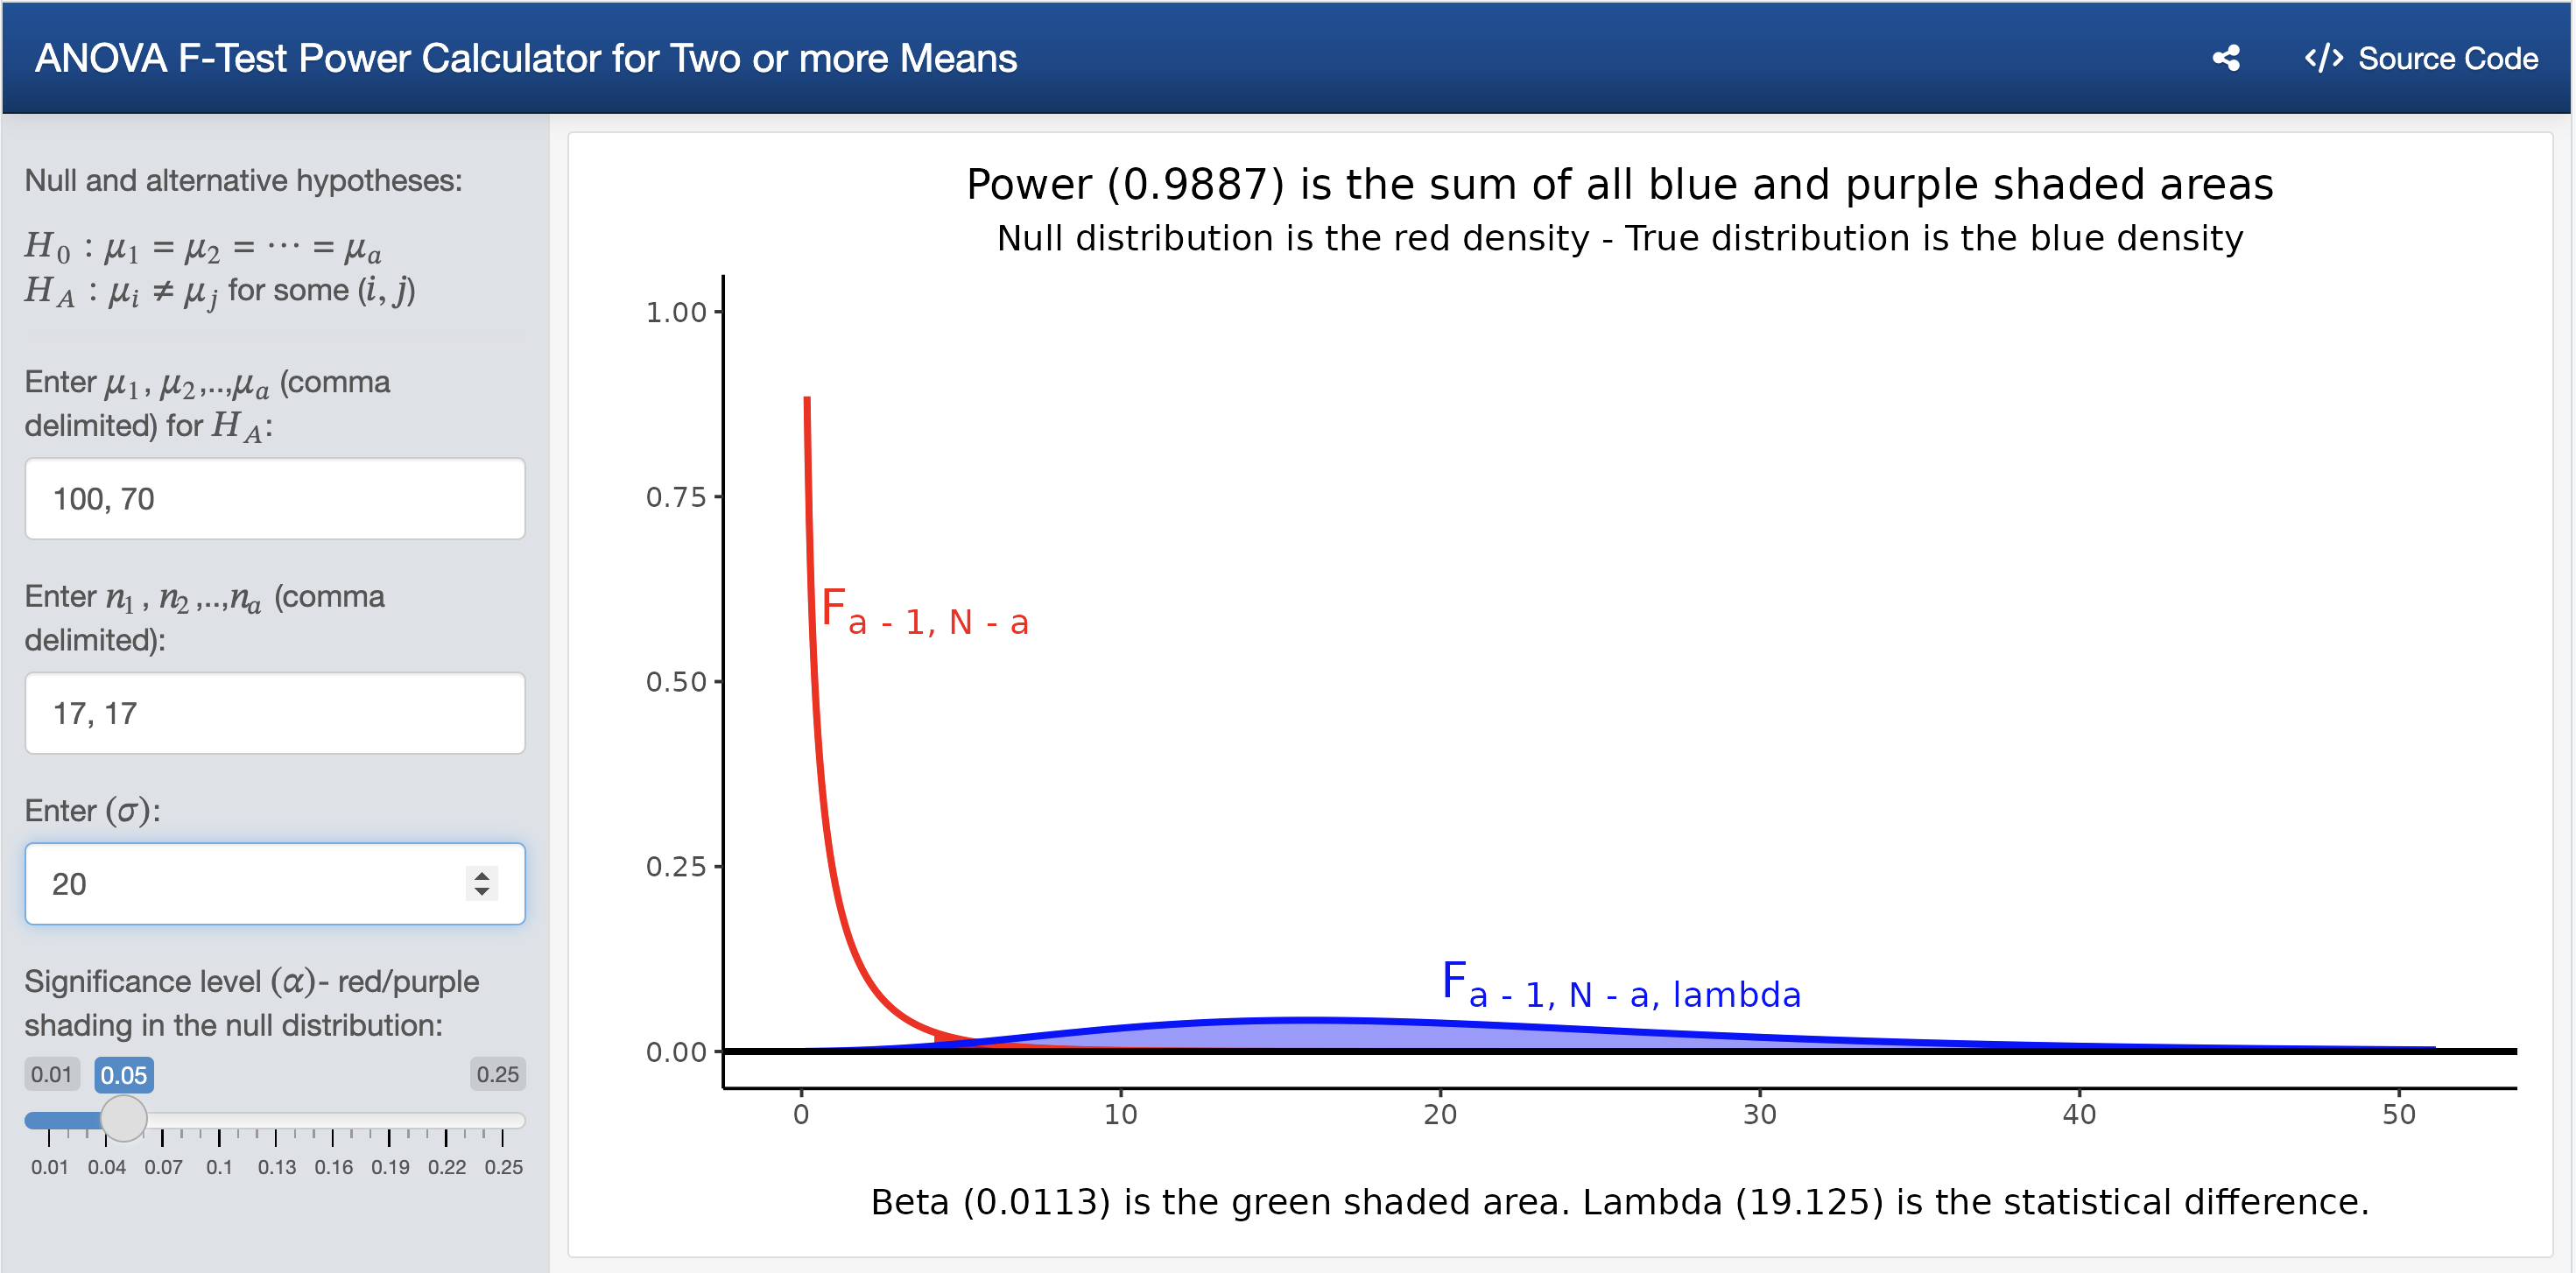
\includegraphics[width=7.36in]{./pics/fig-power1b} 

}

\caption{Power to detect a specified difference in population means with given sample sizes and population standard deviation}\label{fig:power1}
\end{figure}

The red density in Figure \ref{fig:power1} depicts a central \emph{F}-distribution with \(2 - 1 = 1\) and \(17 + 17 - 2 = 32\) degrees of freedom. The blue density in Figure \ref{fig:power1} is a non-central \emph{F}-distribution with \(2-1 = 1\) and \(17 + 17 - 2 = 32\) degrees of freedom and non-centrality parameter (\(\lambda = 19.125)\). The purple shaded area in Figure \ref{fig:power1} is the significance level (all of the area to the right of the critical value 4.1490974 underneath the \emph{F}-distribution) and the sum of all blue and purple shaded areas (all of the area to the right of the critical value 4.1490974 underneath the non-central \emph{F}-distribution) is the power (0.9887). Changing the values for \(n_1\) and \(n_2\) to either 8 and 9 or 9 and 8 results in a power of 0.8224 as shown in Figure \ref{fig:power2}.

\begin{figure}

{\centering 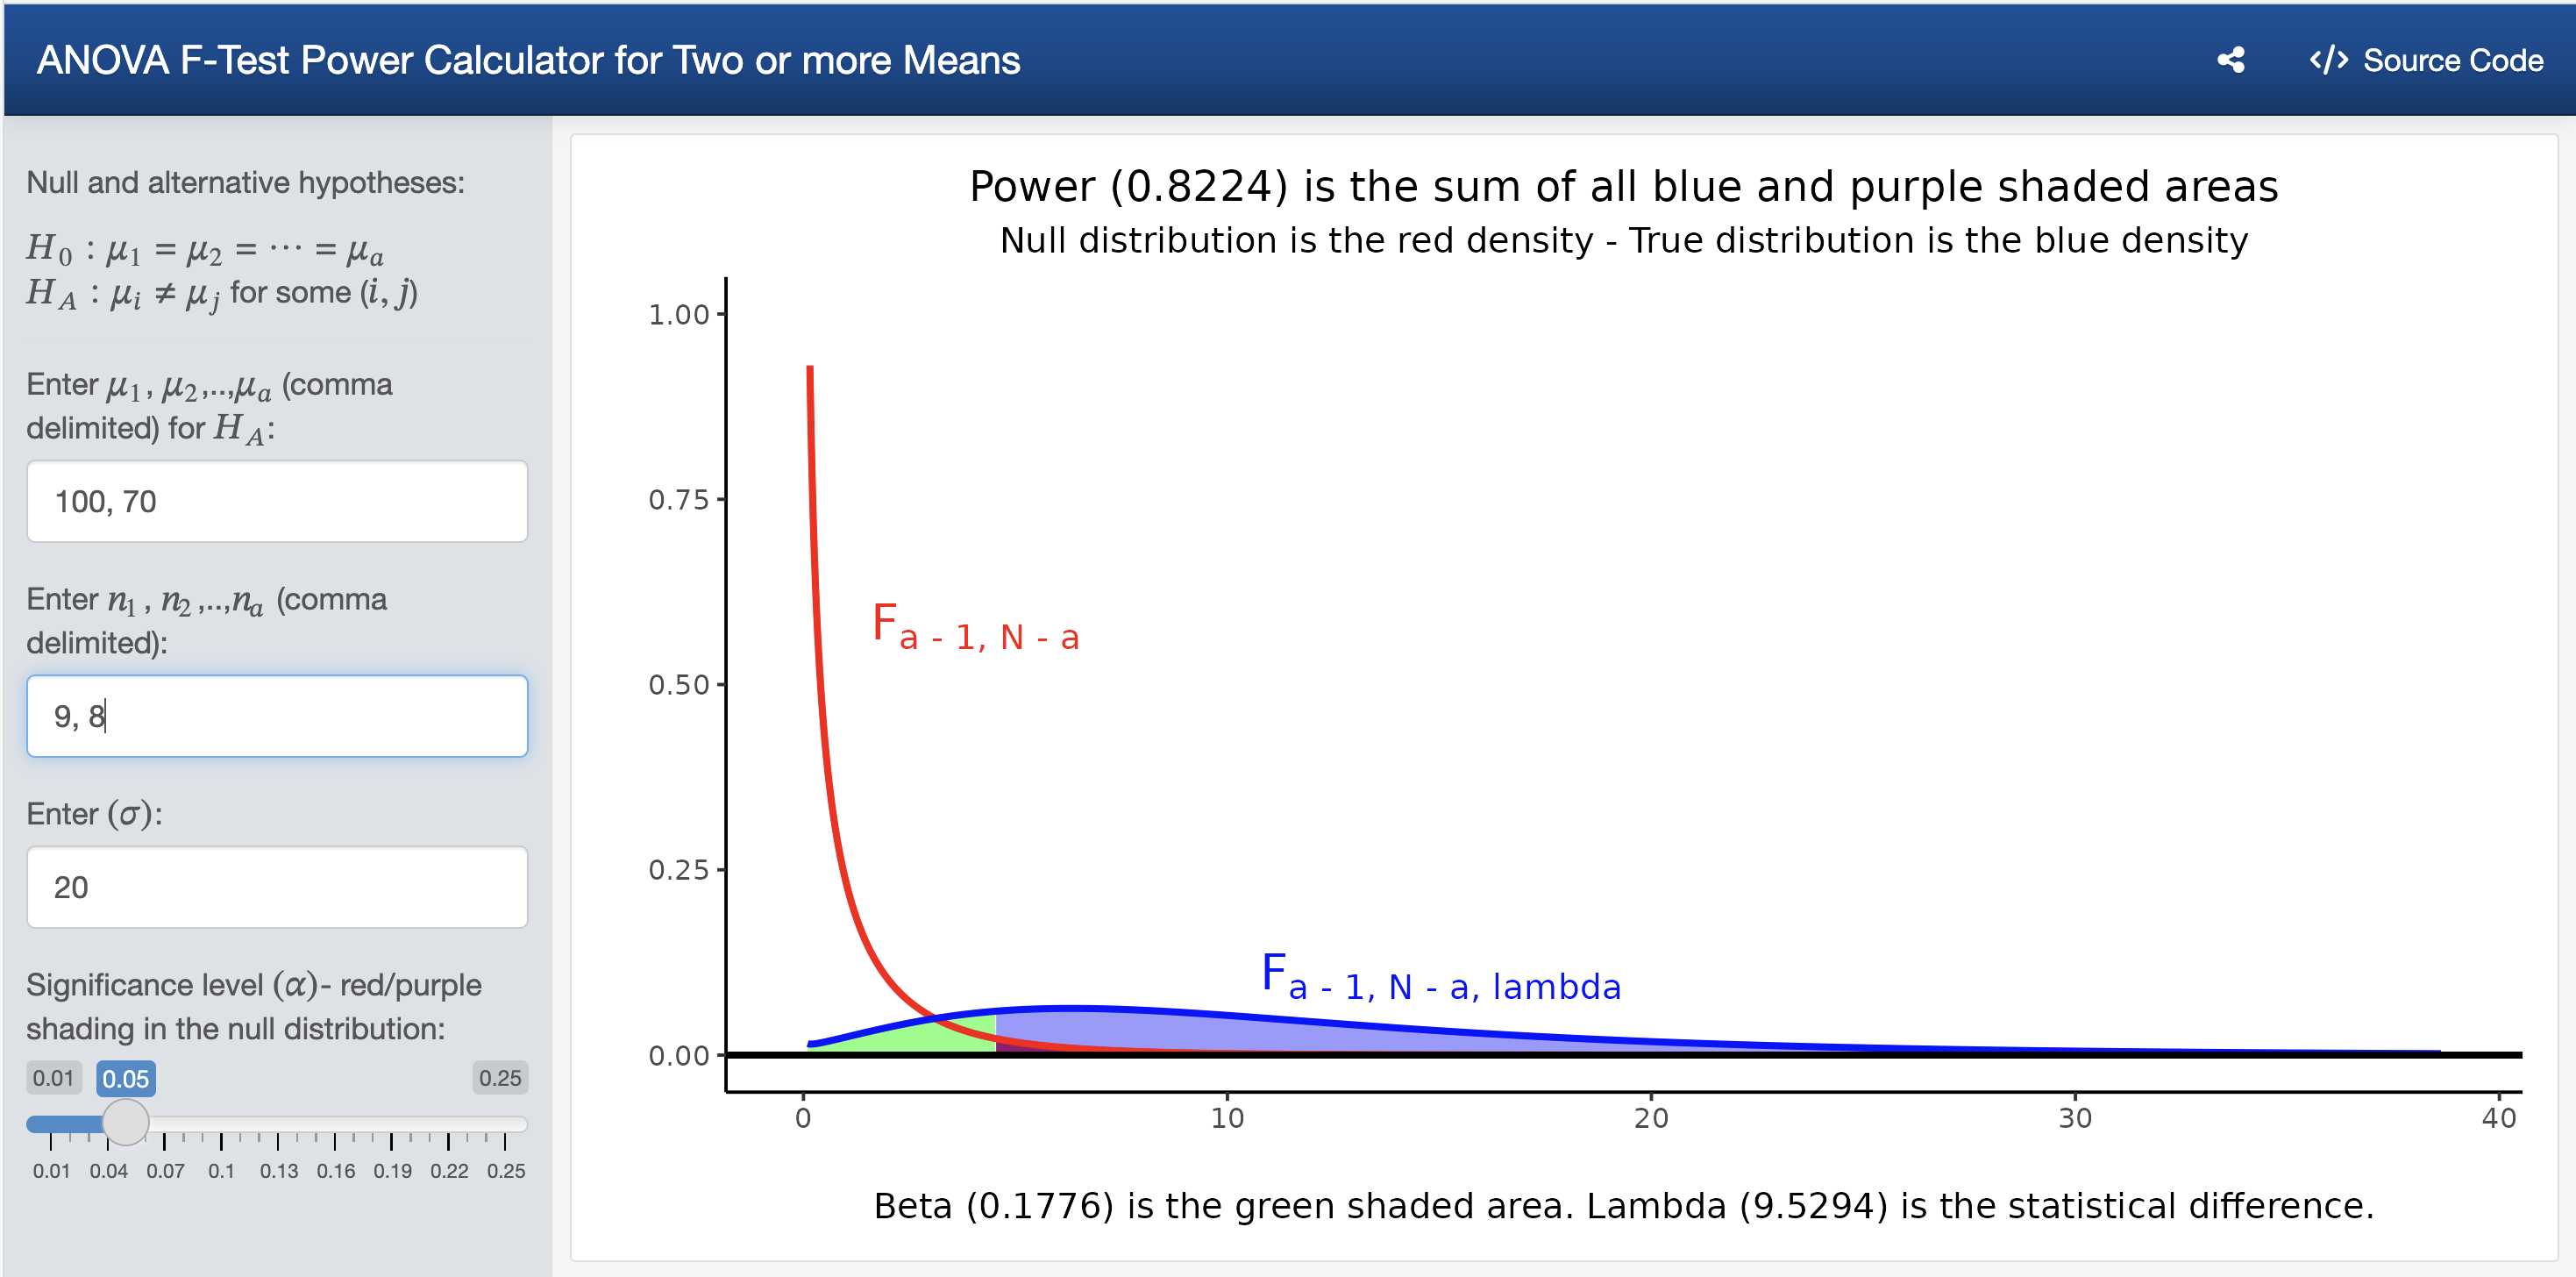
\includegraphics[width=7.34in]{./pics/fig-power2b} 

}

\caption{Power to detect a specified difference in population means with given sample sizes and population standard deviation}\label{fig:power2}
\end{figure}

\subsection*{R code}\label{r-code}
\addcontentsline{toc}{subsection}{R code}

The \texttt{qf()} and \texttt{pf()}, quantile and distribution functions, for the \(F\)-distribution are used to compute the reported quantities in a. and c.~The reader can read the help files for any R function by typing \texttt{?} in front of the function name. In this case, type \texttt{?qf} at the R prompt and press return.

\begin{Shaded}
\begin{Highlighting}[]
\CommentTok{\# Computing critical value}
\NormalTok{CriticalF }\OtherTok{\textless{}{-}} \FunctionTok{qf}\NormalTok{(}\FloatTok{0.95}\NormalTok{, }\DecValTok{2} \SpecialCharTok{{-}} \DecValTok{1}\NormalTok{, }\DecValTok{17} \SpecialCharTok{+} \DecValTok{17} \SpecialCharTok{{-}} \DecValTok{2}\NormalTok{)}
\NormalTok{CriticalF}
\end{Highlighting}
\end{Shaded}

\begin{verbatim}
[1] 4.149097
\end{verbatim}

\begin{Shaded}
\begin{Highlighting}[]
\CommentTok{\# Power for lambda = 19.125}
\NormalTok{POWER }\OtherTok{\textless{}{-}} \FunctionTok{pf}\NormalTok{(CriticalF, }\DecValTok{2} \SpecialCharTok{{-}} \DecValTok{1}\NormalTok{, }\DecValTok{17} \SpecialCharTok{+} \DecValTok{17} \SpecialCharTok{{-}} \DecValTok{2}\NormalTok{, }\FloatTok{19.125}\NormalTok{, }\AttributeTok{lower =} \ConstantTok{FALSE}\NormalTok{)}
\NormalTok{POWER}
\end{Highlighting}
\end{Shaded}

\begin{verbatim}
[1] 0.9886555
\end{verbatim}

\begin{enumerate}
\def\labelenumi{\alph{enumi})}
\setcounter{enumi}{3}
\tightlist
\item
  Have the students use different values for \(n_1 = n_2\) potentially starting with 12 and observing the computed power (0.9394) is more than sufficient. Lead the students through computing the power with reduced sample sizes of \(n_1 = n_2 = 9\) so that the critical value becomes \(f_{1 - \alpha; a - 1, n_1 + n_2 -2} = f_{0.95; 2 - 1, 9 + 9 -2} = f_{0.95; 1, 16} = 4.4939985\) and the non-centrality parameter \(\lambda\) becomes
\end{enumerate}

\begin{equation*}
\lambda = \frac{\sum_{1 = 1}^an_i(\mu_{i\bullet} - \bar{\mu}_{\bullet\bullet})^2}{\sigma^2} = \frac{9(100 - 85)^2 + 9(70 - 85)^2}{20^2} = 10.125.
\end{equation*}

\[\text{Power}(\lambda = 10.125) = P(F^*_{1, 16; \lambda = 10.125} \geq f_{0.95; 1, 16} = 4.4939985) = 0.8476101\]
Next have the students consider \(n_1 = n_2 = 8\) so that the critical value becomes
\(f_{1 - \alpha; a - 1, n_1 + n_2 -2} = f_{0.95; 2 - 1, 8 + 8 -2} = f_{0.95; 1, 14} = 4.6001099\) and the non-centrality parameter \(\lambda\) becomes

\begin{equation*}
\lambda = \frac{\sum_{1 = 1}^an_i(\mu_{i\bullet} - \bar{\mu}_{\bullet\bullet})^2}{\sigma^2} = \frac{8(100 - 85)^2 + 8(70 - 85)^2}{20^2} = 9.
\end{equation*}

\[\text{Power}(\lambda = 9) = P(F^*_{1, 14; \lambda = 9} \geq f_{0.95; 1, 14} = 4.6001099) = 0.796545\]
Since \(n_1 = n_2 = 8\) resulted in a power value less than the required 0.80, the minimum sample size for \(n_1 = n_2\) to obtain a power of at least 0.80 is 9.

e). In this example, \(n_1 = n_2 = 9\) returned a power of 0.8476101 while \(n_1 = n_2 = 8\) returned a power of 0.796545. Although power is maximized when sample sizes are equal, ask the students to use either \(n_1 = 9\) and \(n_2 = 8\) or \(n_1 = 8\) and \(n_2 = 9\) to see if the power is at least 0.80. It does not make a difference whether the first treatment group or the second treatment group receives the smaller number of chicks in computing \(\lambda\) for this problem; however, the value for \(\bar{\mu}_{\bullet\bullet}\) will differ depending on which group receives the smaller number of chicks. The resulting power would be 0.8223981 regardless of whether \(n_1 = 9\) and \(n_2 = 8\) or \(n_1 = 8\) and \(n_2 = 9\). Since the groups are of different sizes, remind the students to weight the means appropriately. That is \(\bar{\mu}_{\bullet\bullet} = \frac{n_1\mu_1+n_2\mu_2}{n_1+n2} =\frac{9\times 100 + 8 \times 70}{9 + 8}=85.88235\) in the case where \(n_1 = 9\) and \(n_2 = 8\) or \(\bar{\mu}_{\bullet\bullet} = \frac{n_1\mu_1+n_2\mu_2}{n_1+n2} =\frac{8\times 100 + 9\times 70}{8 + 9}=84.11765\) in the case where \(n_1 = 8\) and \(n_2 = 9\).

\begin{equation*}
\lambda = \frac{\sum_{1 = 1}^an_i(\mu_{i\bullet} - \bar{\mu}_{\bullet\bullet})^2}{\sigma^2} = \frac{9(100 - 85.88235)^2 + 8(70 - 85.88235)^2}{20^2} = 9.529412
\end{equation*}
or
\begin{equation*}
\lambda = \frac{\sum_{1 = 1}^an_i(\mu_{i\bullet} - \bar{\mu}_{\bullet\bullet})^2}{\sigma^2} = \frac{8(100 - 84.11765)^2 + 9(70 - 84.11765)^2}{20^2} = 9.529412
\end{equation*}

\[\text{Power}(\lambda = 9.529412) = P(F^*_{1, 15, \lambda = 9.529412} \geq f_{0.95, 1, 15} = 4.5430772) = 0.8223981\]

\begin{enumerate}
\def\labelenumi{\alph{enumi})}
\setcounter{enumi}{5}
\tightlist
\item
  The non-centrality parameter when \(\sigma = 30\) mg and \(n_1 = n_2 = 17\) is
\end{enumerate}

\begin{equation*}
\lambda = \frac{\sum_{1 = 1}^an_i(\mu_{i\bullet} - \bar{\mu}_{\bullet\bullet})^2}{\sigma^2} = \frac{17(100 - 85)^2 + 17(70 - 85)^2}{30^2} = \frac{7650}{900} = 8.5
\end{equation*}

\[\text{Power}(\lambda = 8.5) = P(F^*_{1, 32; \lambda = 8.5} \geq f_{0.95; 1, 32} = 4.1490974) = 0.8070367\]
Have the students verify that the minimum samples sizes for \(n_1\) and \(n_2\) are both 17 when \(\sigma = 30\) using the Shiny app as shown in Figure \ref{fig:power3}.

\begin{figure}

{\centering 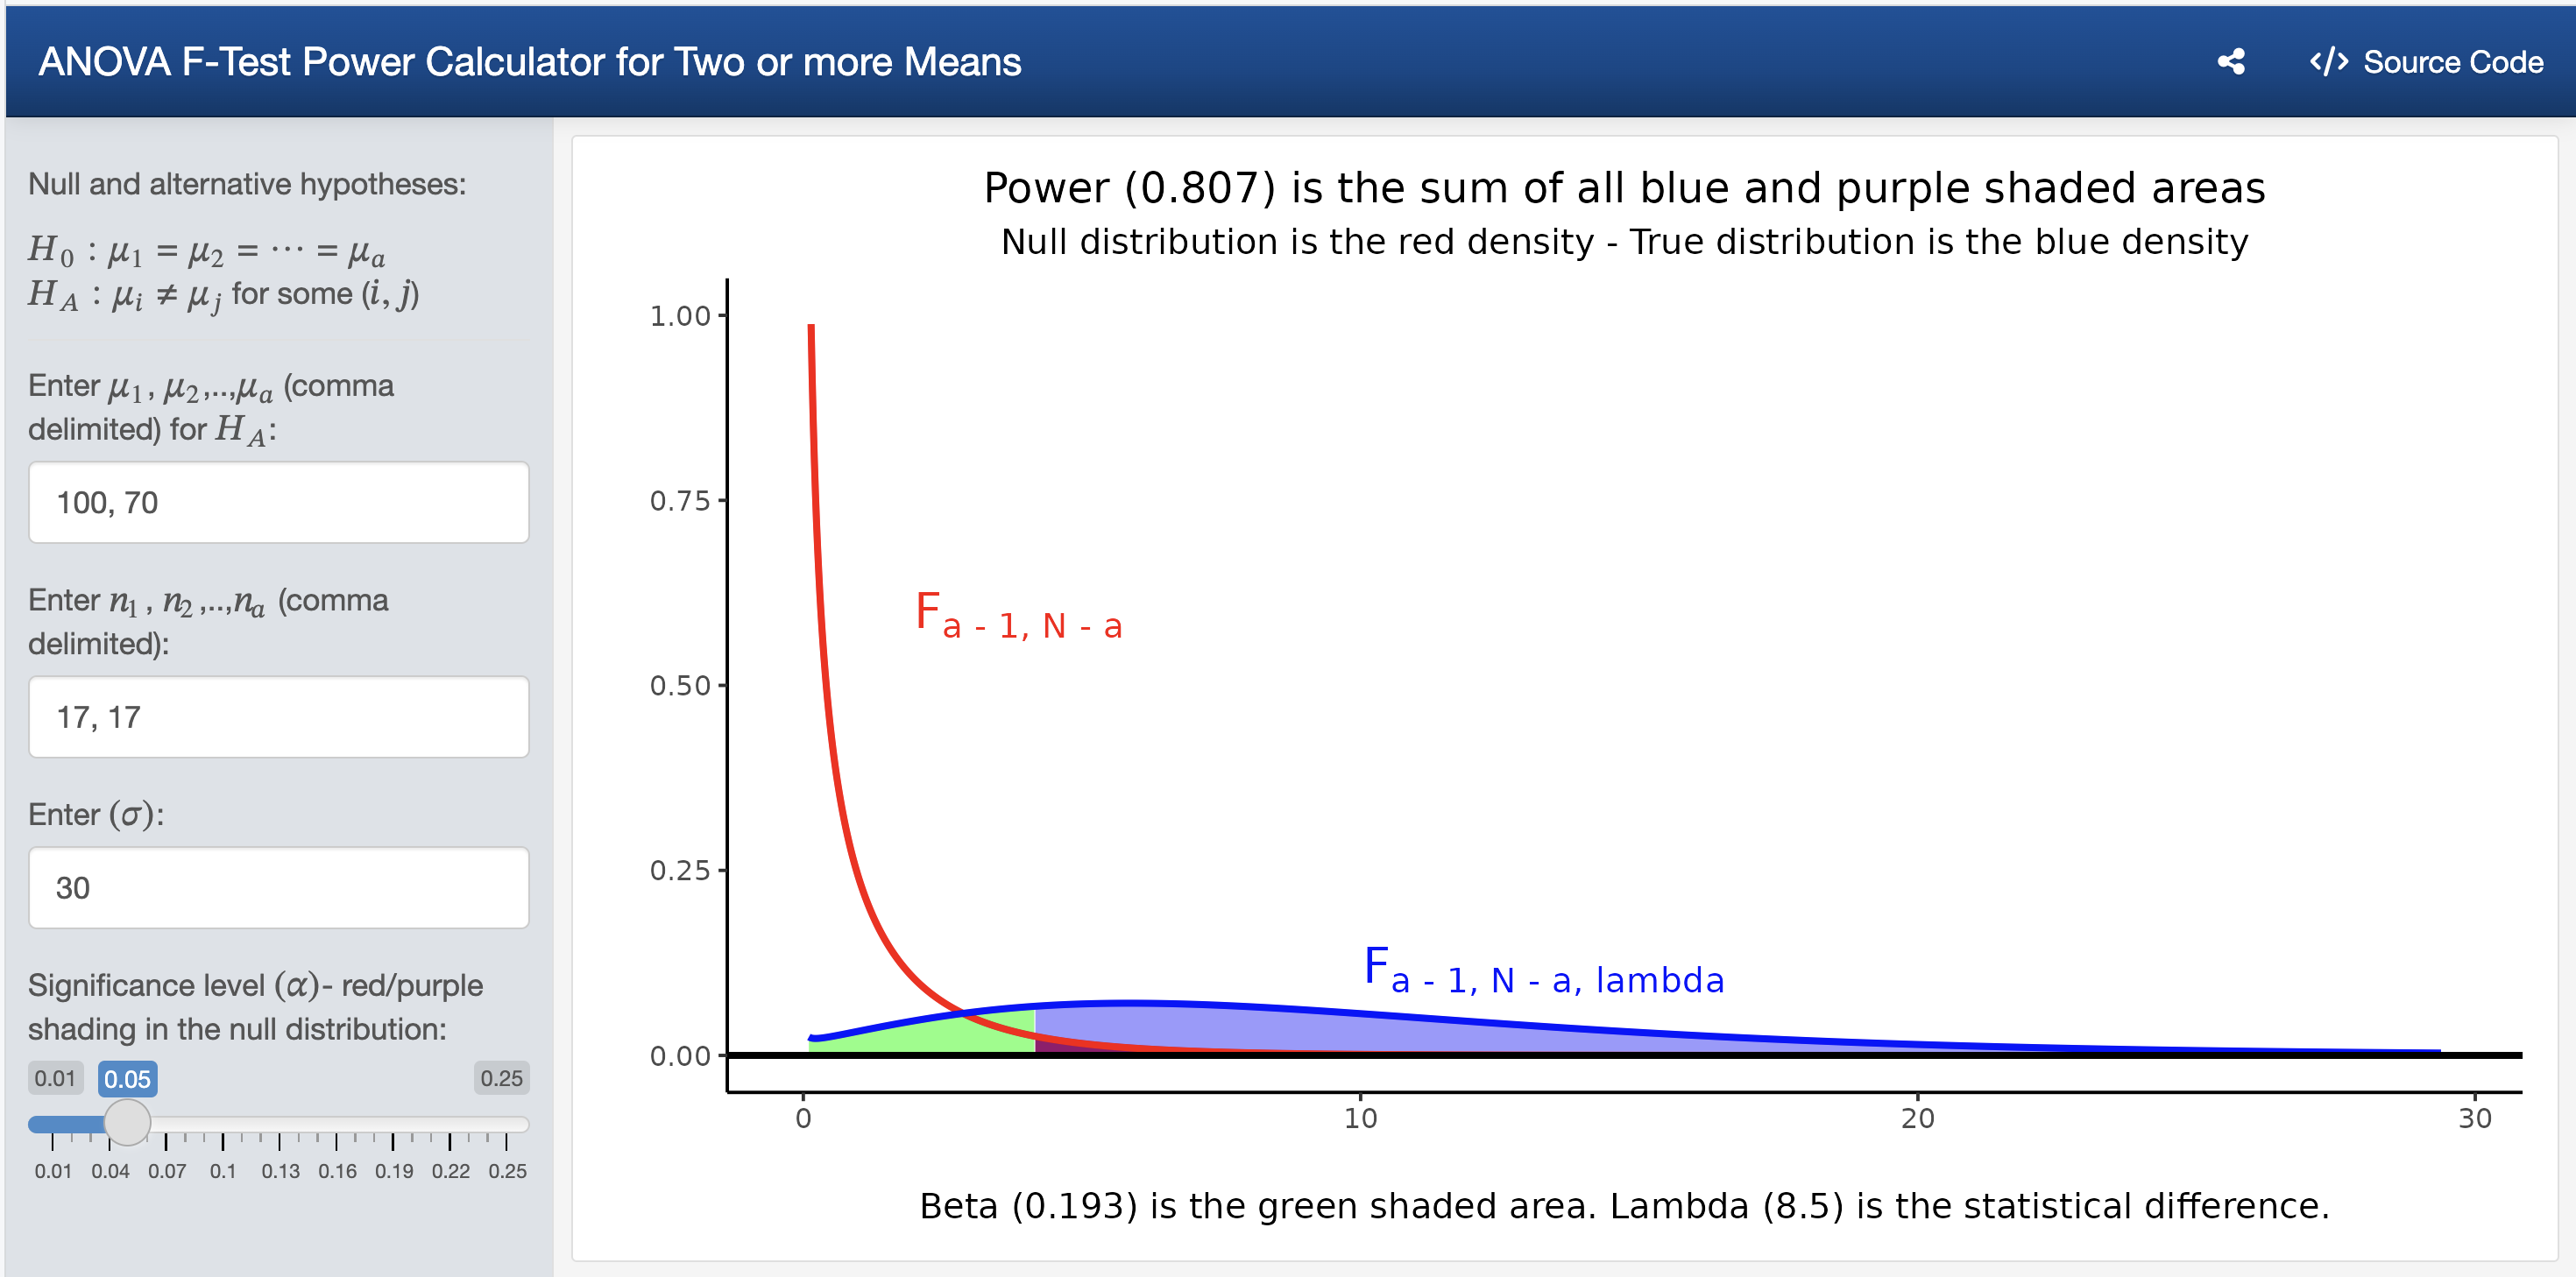
\includegraphics[width=7.35in]{./pics/fig-power3b} 

}

\caption{Power to detect a specified difference in population means with given sample sizes and population standard deviation}\label{fig:power3}
\end{figure}

Note: If the standard deviation for chick weight is \(\sigma = 30\) mg, the student needs to have 17 chicks assigned to each group to detect mean differences between groups greater than 80\% percent of the time. If the standard deviation for chick weights is as small as \(\sigma = 20\) mg, the students can assign 9 chicks to the first group and 8 chicks to the second group and still detect mean differences more than 80\% of the time.

\section*{PROJECT 2}\label{project-2}
\addcontentsline{toc}{section}{PROJECT 2}

An educational researcher is interested in testing different tools to help his students master statistical concepts. The researcher hypothesizes there will be increases in mean performance for students on a standardized test from lecture alone (70), to lecture with statistical software (75), to lecture with statistical software and videos (80), to lecture with statistical software, videos, and shiny apps of (85). If the population standard deviation for the researcher's students on the standardized test is 15, find the minimum number of students required for each group to be able to have a power value of at least 0.80.

To find the required samples sizes to test \(H_0: \mu_1 = \mu_2 = \mu_3 = \mu_4 \quad\text{ versus }\quad H_A: \mu_i \neq \mu_j\) for some \(i \neq j\) using \(\alpha = 0.05\) if in fact \(\mu_1 = 70\), \(\mu_2 = 75\), \(\mu_3 = 80\), and \(\mu_4 = 85\), when \(\sigma = 15\), have the students launch the Shiny app found at \url{https://hasthika.shinyapps.io/anovaShinyApp/} and enter the values of 70, 75, 80, and 85 separated with commas in the \(H_A\) box. Power is maximized when all treatment groups have the same number of experimental units. Consequently, if there are no restrictions on the allocation of resources, students should allocate an equal number of experimental units to each of the \(a\) treatments by entering values separated with commas for each treatment group size in the \(n_1, n_2,\ldots, n_a\) box, the value of 15 in the \(\sigma\) box, and use the slider to select a significance level of 0.05 as shown in Figure \ref{fig:power4}. Have the students experiment with different values for the sample sizes of each treatment until the power is greater than or equal to 0.80. Walk the students through a trial and error method starting with \(n_1 = n_2 = n_3 = n_4 = 10\) which will yield too small a power. As a guess, have the students double the values to \(n_1 = n_2 = n_3 = n_4 = 20\) and point out that we are just a little short of our desired power value. Next, have the students use \(n_1 = n_2 = n_3 = n_4 = 25\) and observe that the returned power is over the target value of 0.80. Have the students continue experimenting lowering the values until they arrive at \(n_1 = n_2 = n_3 = n_4 = 21\) which returns a power of 0.8082.

\begin{table}

\caption{\label{tab:unnamed-chunk-2}Process of trial and error for desired power}
\centering
\begin{tabular}[t]{rr}
\toprule
n & Power\\
\midrule
10 & 0.4396\\
20 & 0.7856\\
25 & 0.8797\\
22 & 0.8287\\
21 & 0.8082\\
\bottomrule
\end{tabular}
\end{table}

\begin{figure}

{\centering 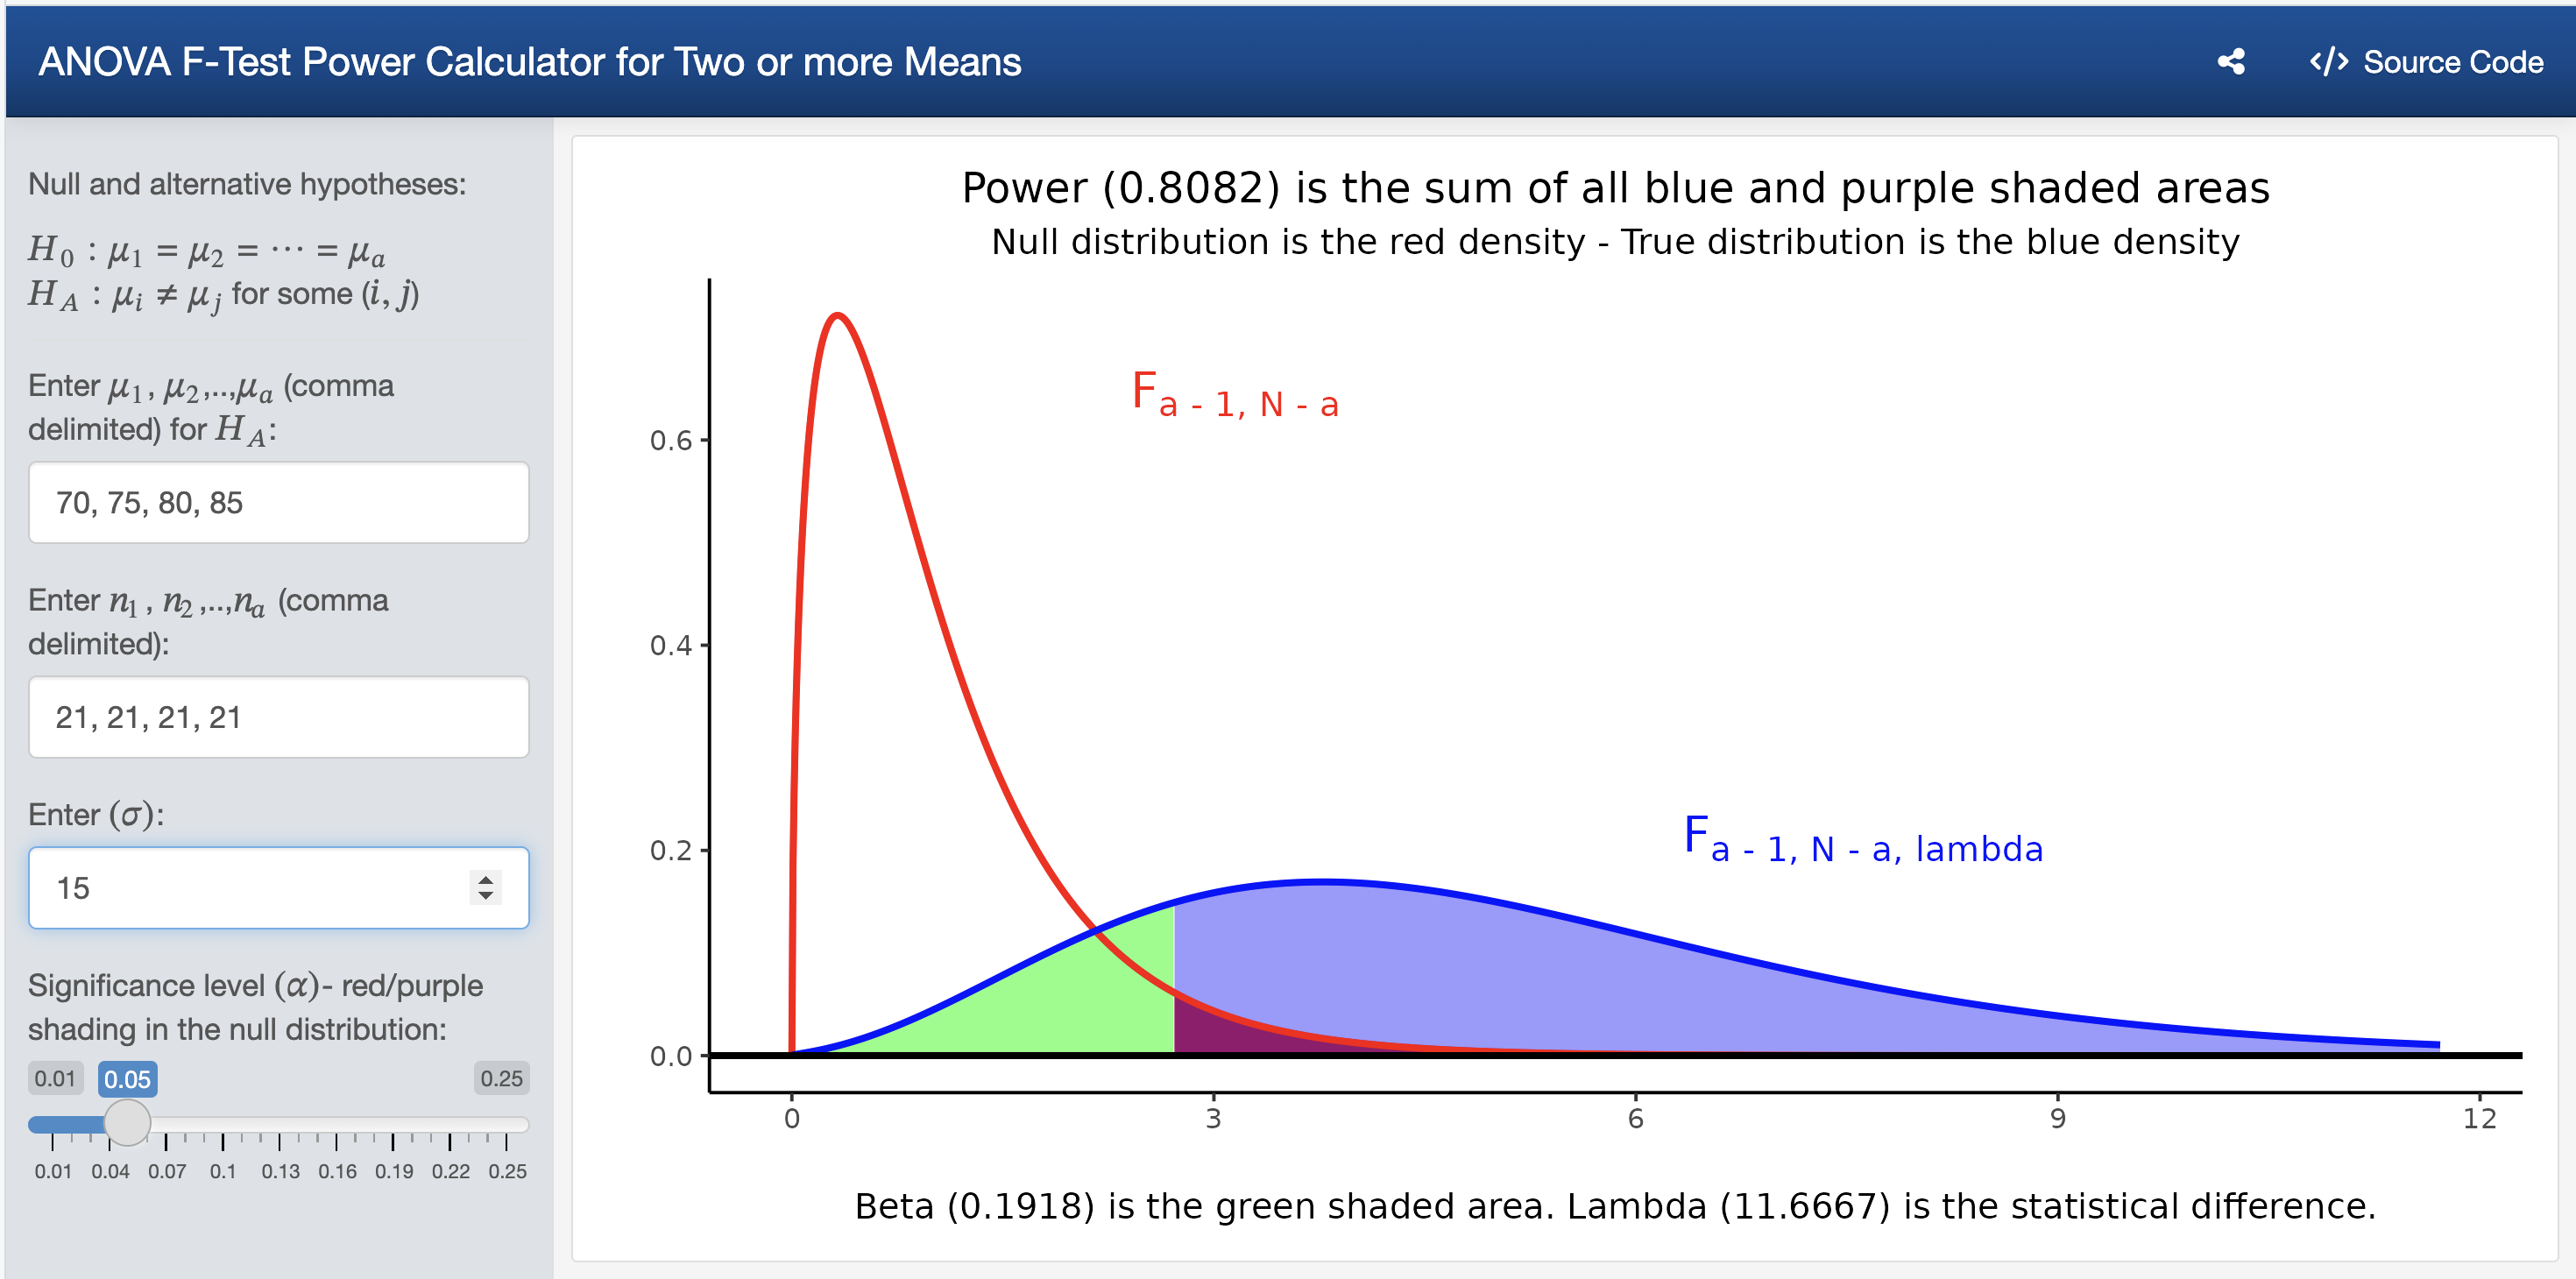
\includegraphics[width=7.35in]{./pics/fig-power4b} 

}

\caption{Power to detect a specified difference in population means with given sample sizes and population standard deviation}\label{fig:power4}
\end{figure}

We note in passing that computing power for full-rank general linear models is also possible using the same paradigm where \(\lambda = \frac{SS_\text{Hypothesis}(\text{population})}{\sigma^2}\). For details see section 12.10 of Ugarte et al. (2015).

\section*{References}\label{references}
\addcontentsline{toc}{section}{References}

\phantomsection\label{refs}
\begin{CSLReferences}{1}{0}
\bibitem[\citeproctext]{ref-arnholtPOWER}
Arnholt, A. T. (2019). Using a shiny app to teach the concept of power. \emph{Teaching Statistics}, \emph{41}(3), 79--84. https://doi.org/\url{https://doi.org/10.1111/test.12186}

\bibitem[\citeproctext]{ref-gaise2016}
Carver, R., Everson, M., Gabrosek, J., Horton, N., Lock, R., Mocko, M., \ldots{} Wood, B. (2016). Guidelines for assessment and instruction in statistics education (GAISE) college report 2016.

\bibitem[\citeproctext]{ref-R-shiny}
Chang, W., Cheng, J., Allaire, J., Sievert, C., Schloerke, B., Xie, Y., \ldots{} Borges, B. (2025). \emph{Shiny: Web application framework for r}. Retrieved from \url{https://shiny.posit.co/}

\bibitem[\citeproctext]{ref-R-base}
R Core Team. (2025). \emph{R: A language and environment for statistical computing}. Vienna, Austria: R Foundation for Statistical Computing. Retrieved from \url{https://www.R-project.org/}

\bibitem[\citeproctext]{ref-snedecor_cochran}
Snedecor, G. W., \& Cochran, W. G. (1967). \emph{Statistical methods, {Sixth} {Edition}}. IOWA State University Press.

\bibitem[\citeproctext]{ref-ugarte_probability_2015}
Ugarte, M. D., Militino, A. F., \& Arnholt, A. T. (2015). \emph{Probability and {Statistics} with {R}, {Second} {Edition}} (2 edition). Boca Raton: Chapman; Hall/CRC.

\end{CSLReferences}

\end{document}
